\documentclass[14pt]{extarticle}
\usepackage{tempora}
\usepackage[T1, T2A]{fontenc}
\usepackage[utf8]{inputenc}
\usepackage[english, ukrainian]{babel}
\usepackage{indentfirst}
\usepackage{geometry}
\usepackage{graphicx}
\usepackage{multirow}
\usepackage{multicol}
\usepackage{float}
\usepackage{listings}
\usepackage{xcolor}
\usepackage{enumitem}
\usepackage{caption}
\usepackage[raggedrightboxes]{ragged2e}
\graphicspath{{/home/artem/Pictures}}
\geometry
{
    a4paper,
    left=20mm,
    top=20mm,
    right=10mm,
    bottom=20mm,
}
\captionsetup[figure]{labelsep=period}



\begin{document}
\begin{titlepage}
    \begin{center}
        \textbf{\normalsize{\MakeUppercase{
            Міністерство Освіти і науки України
            Національний університет "Львівська політехніка"
        }}}

        \begin{flushright}
        \textbf{ІКНІ}\\
        Кафедра \textbf{ПЗ}
        \end{flushright}
        \vspace{15mm}

        %\includegraphics[width=0.4\textwidth]{lpnu_logo.png}

        \vspace*{\fill}

        \textbf{\normalsize{\MakeUppercase{Курсова Робота}}}
            

        \textbf{на тему:} “ Автомобільна дорога”

        \textbf{з дисципліни:} “Об'єктно орієнтовне програмування”
            
        \vspace*{\fill}

        \begin{flushright}

            Стедента групи   ПЗ-24\\

            \vspace*{12pt}
            спеціальності 6.121\\

            \vspace*{12pt}
            “Інженерія програмного забезпечення”\\

            \vspace*{12pt}
            Губика Артема\\

            \vspace*{12pt}
            Керівник: доцент кафедри ПЗ,

            \vspace*{12pt}
            к.т.н., доцент Коротєєва Т. О.

            \vspace*{12pt}
            \rule{3cm Національна шкала\space}{0.3pt} 

            \vspace*{12pt}
            \rule{0.40cm Кількість балів\space}{0.3pt} 
            \rule{0.4cm Оцінка ECTS\space}{0.3pt} 

            Члени комісії
            \rule{2.5cm  \space}{0.3pt} 
            \rule{7cm \space}{0.3pt} 

            \rule{2.5cm  \space}{0.3pt} 
            \rule{7cm \space}{0.3pt} 

            \rule{2.5cm  \space}{0.3pt} 
            \rule{7cm \space}{0.3pt} 
        \end{flushright}

        \vspace*{24pt}
        Львів -- 2023
            
            
    \end{center}
\end{titlepage}

% --- Зміст ---%
\tableofcontents
\break
% --- Зміст ---%


\section{Завдання до курсової роботи}

Варіант 3:
Створити клас Дорога

Автомобільна дорога | Тип (державна/регіональна/обласна/місцева) |  Протяжність | Кількість смуг |  Наявність пішохідної доріжки |  Наявність розділювача посередині дороги
\begin{enumerate}
\item Впорядкувати дороги за протяжністю.
\item Знайти найкоротшу дорогу, де найбільша кількість смуг.
\item Знайти всі дороги, в яких наявні розділювачі посередині, кількість смуг >2 та згрупувати за типом.
\item Визначити типи автомобільних доріг, з найбільшою протяжністю та наявністю пішохідних доріжок.
\item Визначити автомобільні дороги з найбільшою кількістю смуг та наявними пішохідними доріжками які належать до регіональних.
\end{enumerate}
Для класу створити:
\begin{enumerate}
\item Конструктор за замовчуванням;
\item Конструктор з параметрами; 
\item конструктор копій; 
\item перевизначити операції >>, << для зчитування та запису у файл. Для демонстрації роботи програми використати засоби візуального середовища програмування.

\begin{center}
    \begin{tabular}{| c | p{13cm} | c | }
        \hline
        \textnumero{} з/п & Зміст завдання & Дата\\
        \hline
        1 &
Здійснити аналiтичний огляд лiтератури за заданою темою та обгрунтувати вибір інструментальних засобів реалізації.
&
08.10 \\
        \hline
2 &
Побудова UML діаграм &
08.10\\
        \hline
        3 &
Розробка алгоритмів реалізації &
11.10 \\

        \hline
        4 &
Реалізація завдання (кодування) &
21.10\\

        \hline
        5 &
Формування інструкції користувача &
25.10 \\

        \hline

6 &

Оформлення звіту до курсової роботи згідно з вимогами Міжнародних стандартів, дотримуючись такої структури:

% ___________________ 
% 						        
% _______________
%__________20.09.2023__
%
\begin{itemize}
    
\item Оформлення звіту до курсової роботи згідно з вимогами Міжнародних стандартів, дотримуючись такої структури:
\item зміст;
\item алгоритм розв‘язку задачі у покроковому представленні;
\item діаграми UML класів, прецедентів, послідовності виконання;
\item код розробленої програми з коментарями;
\item протокол роботи програми для кожного пункту завдання
\item інструкція користувача та системні вимоги;
\item опис виняткових ситуацій;
\item структура файлу вхідних даних;
\item висновки;
\item список використаних джерел.

\end{itemize}
&
05.11\\
        \hline




        
    \end{tabular}
    
\end{center}
\end{enumerate}

\rule{3cm Завдання прийнято до виконання:\space}{0.3pt} 
(Губик А. С.)

\hspace{7.4cm} \textsuperscript{( пiдпис студента )}

\rule{3cm Керівник роботи:\space}{0.3pt} 
( Коротєєва Т. О.)

%\rule{3cm Дата видачі завдання\space}{0.3pt} 
Дата видачі завдання: \underline{20.09.2023}

\break
\section{Алгоритм розв‘язку задачі у покроковому представленні}

\subsection{Сортування доріг за протяжністю (Sort by Length -- SBL)}

\newlist{firstlist}{enumerate}{2}
\setlist[firstlist, 1]{label=SBL\arabic{firstlisti},
leftmargin=20mm,
rightmargin=10pt}
\setlist[firstlist, 2]{label=SBL\arabic{firstlisti}.\arabic{firstlistii}}

\begin{firstlist}
\item Порівняння елементів і обмін:
        \begin{firstlist}
        \item Порівняємо перший елемент з наступним.
        \item Якщо довжина першої дороги більша за довжину наступної, міняємо їх місцями.
        \item Перше порівняння: (Roads[0] > Roads[1])
        \end{firstlist}

\item Перший прохід по списку:
\begin{firstlist}
    
        \item Продовжуємо порівнювати та міняти місцями сусідні елементи.
        \item Довжина доріг порівнюється і міняється за необхідності.
        \item Кінець першого проходу: найбільший елемент (за довжиною) розміщується в кінці списку.
\end{firstlist}

\item Повторення ітерацій:
\begin{firstlist}
    
        \item Процес повторюється для усього списку, крім вже відсортованих елементів.
        \item З кожною ітерацією найбільший (за довжиною) елемент "спливає" до кінця списку.
\end{firstlist}

\item Фінальна ітерація:
\begin{firstlist}
        \item Повний прохід відбувається до тих пір, поки всі елементи не будуть відсортовані за зростанням довжини.
        \item Кінцевий результат: список доріг, відсортований за зростанням довжини.
\end{firstlist}
\end{firstlist}

\subsection{Знайти найкоротшу дорогу, де найбільша кількість смуг. (Shortest road  most lanes -- SRML)}

\newlist{secondList}{enumerate}{2}
\setlist[secondList, 1]{label=SRML\arabic{secondListi},
leftmargin=20mm,
rightmargin=10pt}
\setlist[secondList, 2]{label=SRML\arabic{secondListi}.\arabic{secondListii}}

\begin{secondList}
\item Очистка списку RequestedRoads:
\begin{secondList}
    
\item Починаємо з очищення списку RequestedRoads, щоб гарантувати, що він буде порожнім перед початком операцій.
\end{secondList}

\item Перевірка умови наявності доріг:
\begin{secondList}
    
\item Перевірка наявності доріг в колекції Roads або її порожності.
\item Якщо Roads не існує або він порожній, функція завершується і повертає порожній список RequestedRoads.
\end{secondList}

\item Пошук дороги з найменшою довжиною та найбільшою кількістю смуг:
\begin{secondList}
\item Ініціалізація змінних для зберігання найменшої довжини та найбільшої кількості смуг дороги.
\item Перебір всіх доріг у колекції та знаходження дороги з найменшою довжиною.
\item Якщо зустрічаємо дорогу із меншою довжиною, оновлюємо значення довжини та кількості смуг, а також вибираємо цю дорогу.
\end{secondList}

\item Додавання вибраної дороги до RequestedRoads:
\begin{secondList}
\item Додаємо вибрану дорогу із найменшою довжиною та, можливо, найбільшою кількістю смуг до списку RequestedRoads.
\end{secondList}

\item Зміна візуальної видимості (SecondTaskVisible):
\begin{secondList}
\item Змінюємо властивість SecondTaskVisible для відображення або приховання пов'язаних з цим елементів інтерфейсу користувача. 
\end{secondList}
\end{secondList}
\subsection{Знайти всі дороги, в яких наявні розділювачі посередині, кількість смуг >2 та згрупувати за типом. (A Complex One -- ACO)}

\newlist{thirdList}{enumerate}{2}
\setlist[thirdList, 1]{label=ACO\arabic{secondListi},
leftmargin=20mm,
rightmargin=10pt}
\setlist[thirdList, 2]{label=ACO\arabic{secondListi}.\arabic{secondListii}}

\begin{thirdList}
\item Очищення списку RequestedRoads:
\begin{thirdList}
\item Починаємо з очищення списку RequestedRoads, щоб гарантувати, що він буде порожнім перед виконанням нових операцій.
\end{thirdList}

\item Перевірка наявності доріг:
\begin{thirdList}
\item Перевірка, чи існують дороги в колекції Roads або чи вона порожня.
\item Якщо Roads не існує або вона порожня, функція завершується, повертаючи порожній список RequestedRoads.
\end{thirdList}

\item Пошук доріг із певними умовами:
\begin{thirdList}
\item Перебираємо всі дороги в колекції.
\item Якщо зустрічаємо дорогу, де кількість смуг більша за 2 і є лінія, додаємо цю дорогу до списку RequestedRoads.
\end{thirdList}

\item Зміна візуальної видимості (SecondTaskVisible):
\begin{thirdList}
\item Змінюємо властивість SecondTaskVisible для відображення або приховання пов'язаних з цим елементів інтерфейсу користувача.
\end{thirdList}

\end{thirdList}
\subsection{Визначити тип автомобільних доріг, з найбільшою протяжністю та наявністю пішохідних доріжок. (Heighest length and pavement -- HLP)}

\newlist{fourthList}{enumerate}{2}
\setlist[fourthList, 1]{label=HLP\arabic{fourthListi},
leftmargin=20mm,
rightmargin=10pt}
\setlist[fourthList, 2]{label=HLP\arabic{fourthListi}.\arabic{fourthListii}}

\begin{fourthList}
\item Перевірка наявності доріг:
\begin{fourthList}
    
    \item Перевірка, чи Roads не порожній і не має значення null.
    \item Якщо Roads не існує або вона порожня, функція завершується, не виконуючи подальших дій.
\end{fourthList}

\item Пошук типу доріг з певними умовами:
\begin{fourthList}
    \item Визначаємо початкові значення: тип selectedType встановлено як RoadType.National (припускаючи значення за замовчуванням).
    \item Шукаємо серед всіх доріг ті, у яких є покриття (HasPavement) і довжина більша за maxLength.
    \item Якщо знаходимо дорогу, що відповідає умовам, оновлюємо selectedType на тип цієї дороги.
\end{fourthList}

\item Виведення результату в консоль:
\begin{fourthList}
    \item Після завершення пошуку виводимо у консоль тип доріг із найбільшою довжиною та наявним покриттям (HasPavement). 
\end{fourthList}

    
\end{fourthList}
\subsection{Визначити автомобільні дороги з найбільшою кількістю смуг та наявними пішохідними доріжками які належать до регіональних.(Regional most lane and pavement -- RMLP)}

\newlist{fifthList}{enumerate}{2}
\setlist[fifthList, 1]{label=RMLP\arabic{fifthListi},
leftmargin=20mm,
rightmargin=10pt}
\setlist[fifthList, 2]{label=RMLP\arabic{fifthListi}.\arabic{fifthListii}}

\begin{fifthList}
    
    
\item Очищення списку RequestedRoads:
\begin{fifthList}
\item Починаємо з очищення списку RequestedRoads, щоб гарантувати його порожність перед подальшою роботою.
\end{fifthList}

\item Перевірка наявності доріг:
\begin{fifthList}
\item Перевіряємо, чи Roads не порожній і не є null. Якщо це так, функція завершується, не виконуючи подальших дій.
\end{fifthList}

\item Пошук доріг з певними умовами:
\begin{fifthList}
\item Шукаємо серед всіх доріг ті, які мають більше двох смуг та наявну пішохідну доріжку (pavement).
\item Додаємо ці дороги до списку RequestedRoads.
\end{fifthList}

\item Зміна візуальної видимості SecondTaskVisible:
\begin{fifthList}
\item Змінюємо властивість SecondTaskVisible для відображення або приховання елементів інтерфейсу, що пов'язані з наступною дією користувача.
\end{fifthList}

\end{fifthList}

\section{Діаграми UML класів, прецедентів, послідовності виконання.}
\begin{figure}[H]
    \centering
    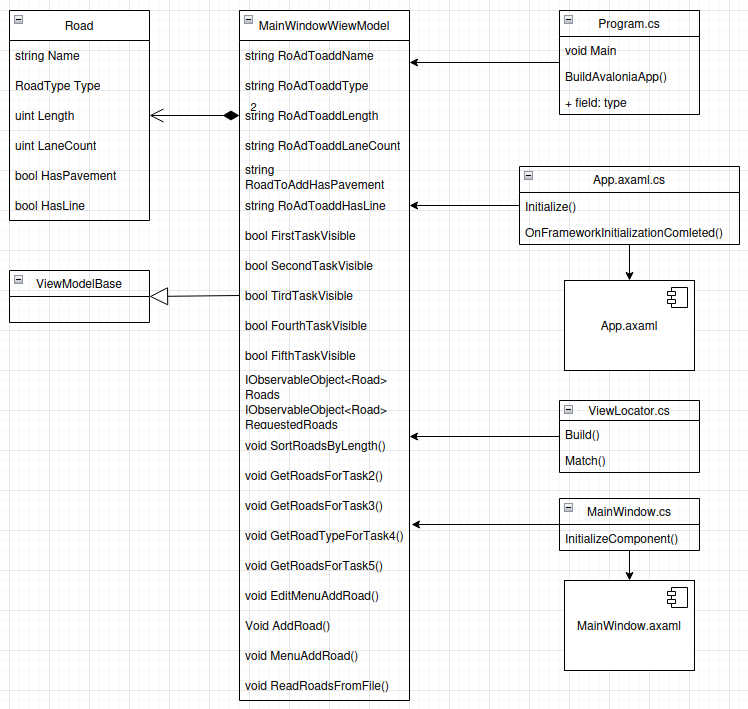
\includegraphics[width=0.90\textwidth]{class_diagram}
    \caption{UML діаграма класів}
\end{figure}
\begin{figure}[H]
    \centering
    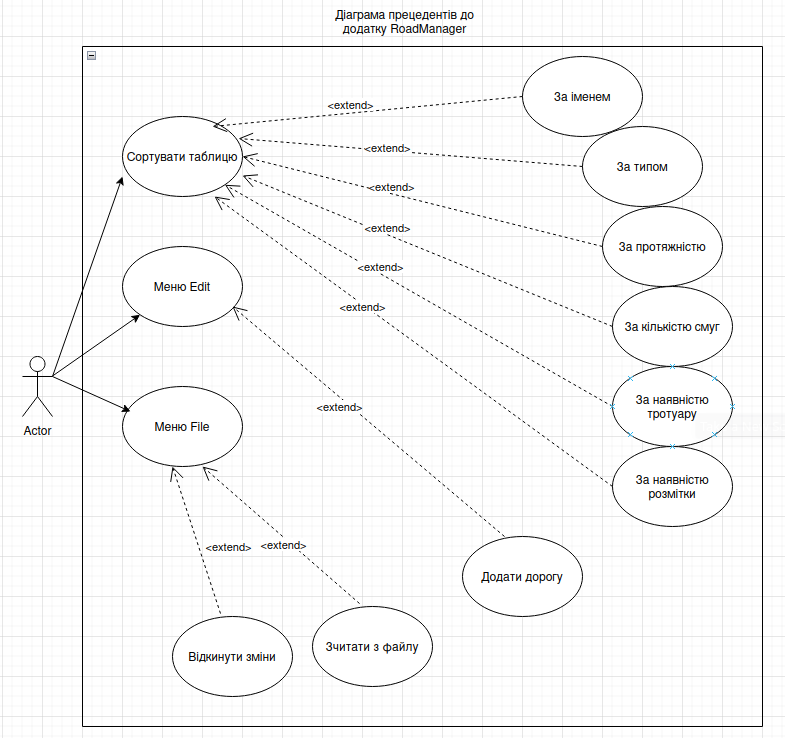
\includegraphics[width=0.90\textwidth]{actor}
    \caption{Діаграма прецедентів}
\end{figure}
\begin{figure}[H]
    \centering
    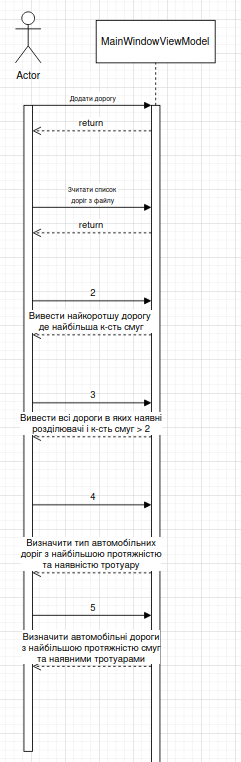
\includegraphics[width=0.50\textwidth]{sequence}
    \caption{Діаграма послідовностей}
\end{figure}

\section{Код розробленої програми з коментарями}
%\lstdefinestyle{sharpc}{language=[Sharp]C, frame=lr, rulecolor=\color{blue!80!black}}
%\lstset{style=sharpc}
\subsection{Road.cs:}
\begin{verbatim}
    namespace RoadClass
    {
        public enum RoadType
        {
            National,
            Regional,
            Oblast,
            Local
        
        }
        public class Road
        {
            public string? Name{get; set;} = "Noname";
    
            public RoadType Type{get; set;} = RoadType.Local;
            public uint Length{get; set;}  = 1;
            public uint LaneCount{get; set;} = 1;
            public bool HasPavement{get; set;} = false;
            public bool HasLine{get; set;} = false;
    
            public Road(string name, RoadType type, uint length, uint laneCount, bool hasPavement, bool hasLine){
                Name = name;
                Type = type;
                Length = length;
                LaneCount = laneCount;
                HasPavement = hasPavement;
                HasLine = hasLine;
            }
            public Road(Road other){
                Name = other.Name;
                Type = other.Type;
                Length = other.Length;
                LaneCount = other.LaneCount;
                HasPavement = other.HasPavement;
                HasLine = other.HasLine;
            }
    
    
            public Road(){}
        }
    }
\end{verbatim}

\subsection{MainWindow.cs:}
\begin{verbatim}
    using Avalonia.Controls;
    using RoadManager.ViewModels;
    
    namespace RoadManager.Views;
    
    public partial class MainWindow : Window
    {
        public MainWindow()
        {
            InitializeComponent();
            DataContext = new MainWindowViewModel();
            
        }
    }
    
\end{verbatim}

\subsection{MainWindow.axaml:}
\begin{verbatim}
<Window xmlns="https://github.com/avaloniaui"
xmlns:x="http://schemas.microsoft.com/winfx/2006/xaml"
xmlns:d="http://schemas.microsoft.com/expression/blend/2008"
xmlns:mc="http://schemas.openxmlformats.org/markup-compatibility/2006"
mc:Ignorable="d" d:DesignWidth="800" d:DesignHeight="450"
x:Class="KurSUCH.MainWindow"
Title="KurSUCH"
Background="#dedede">

<Grid RowDefinitions="Auto, Auto, *">
    <Grid Grid.Row="0" Background="White" Height="30" ColumnDefinitions="Auto, Auto, Auto, *">
        <Button Grid.Column="0" Content="File" Foreground="Black"/>
        <Button Grid.Column="1" Content="Edit" Foreground="Black"/>
        <Button Grid.Column="2" Content="Help" Foreground="Black"/>
        <Rectangle></Rectangle>
    </Grid>
    <Grid Grid.Row="1" Background="#dedede" Height="50" ColumnDefinitions="Auto, Auto, Auto, *">
        <Button Grid.Column="0">
            <Image Source="/Assets/plus.png" />
        </Button>
        <Button Grid.Column="1">
            <Image Source="/Assets/error.png" />
        </Button>
        <Button Grid.Column="2">
            <Image Source="/Assets/error.png" />
        </Button>
        <Rectangle Grid.Column="3" Fill="Black" />
    </Grid>
    <Grid ColumnDefinitions="*, Auto">
        <DataGrid Grid.Column="0" ItemsSource="Binding Roads">
                <DataGrid.Columns>
                <DataGridTextColumn Header="Name" 
                                    Binding="{Binding Name}" 
                                    Width="2*" />
                <DataGridTextColumn Header="Last Name" 
                                    Binding="{Binding Type}" 
                                    Width="*" />
                <DataGridTextColumn Header="Department" 
                                    Binding="{Binding Length}" 
                                    Width="*" />
                <DataGridTextColumn Header="Department" 
                                    Binding="{Binding LaneCount}" 
                                    Width="*" />
                <DataGridTextColumn Header="Department" 
                                    Binding="{Binding HasPavement}" 
                                    Width="*" />
                <DataGridTextColumn Header="Department" 
                                    Binding="{Binding HasLine}" 
                                    Width="*" />
                </DataGrid.Columns>
        </DataGrid>
    </Grid>
</Grid>

</Window>

\end{verbatim}
\subsection{MainWindowViewModel.cs:}
\begin{verbatim}
using System;
using System.IO;
using System.Linq;
using System.Collections.Generic;
using System.Collections.ObjectModel;
using System.ComponentModel.DataAnnotations;

using System.Diagnostics;
using System.Reactive;
using System.Text;
using ReactiveUI;
using RoadClass;
using Avalonia;
using Avalonia.Controls;
using Avalonia.Markup.Xaml;
using RoadManager.Views;
namespace RoadManager.ViewModels;

public class MainWindowViewModel : ViewModelBase
{
    private string _RoadToAddName = "Name";
    private uint _RoadToAddTypeIndex;
    private RoadType _RoadToAddType;
    private uint _RoadToAddLength;
    private uint _RoadToAddLaneCount;
    private bool _RoadToAddHasPavement;
    private bool _RoadToAddHasLine;
    private string _MenuOpenFileText = "in.txt";

    [Required]
    public string MenuOpenFileText
    {
        get => _MenuOpenFileText;
        set => this.RaiseAndSetIfChanged(ref _MenuOpenFileText, value);
    }
    //private string _RoadToAddName;

    public uint RoadToAddTypeIndex
    {
        get => _RoadToAddTypeIndex; 
        set => this.RaiseAndSetIfChanged(ref _RoadToAddTypeIndex, value);
    }
    public uint RoadToAddLaneCount
    {
        get => _RoadToAddLaneCount; 
        set => this.RaiseAndSetIfChanged(ref _RoadToAddLaneCount, value);
    }
    public uint RoadToAddLength
    {
        get => _RoadToAddLength; 
        set => this.RaiseAndSetIfChanged(ref _RoadToAddLength, value);
    }
    [Required]
    public string RoadToAddName
    {
        get => _RoadToAddName;
        set
        {
        if(value == "")
        {
            //throw new ArgumentNullException("", "This field is required");
        }
        this.RaiseAndSetIfChanged(ref _RoadToAddName, value);
        }
    }
    public bool RoadToAddHasPavement
    {
        get => _RoadToAddHasPavement;
        set => this.RaiseAndSetIfChanged(ref _RoadToAddHasPavement, 
                                        _RoadToAddHasPavement ^= true);
    }
    public bool RoadToAddHasLine
    {
        get => _RoadToAddHasLine;
        set => this.RaiseAndSetIfChanged(ref _RoadToAddHasLine, 
                                        _RoadToAddHasLine ^= true);
    }
    
    //private bool[] ItemVisibility = new bool[10];

    public ObservableCollection<bool> ItemVisibility { get; } = new ObservableCollection<bool>(Enumerable.Repeat(false, 10));


    public bool AddRoadVisible
    {
        get => ItemVisibility[0];
        set
        { 
            for(int i = 0; i < ItemVisibility.Count; i++){
                ItemVisibility[i] = false;
            }
            ItemVisibility[0] = true; 
        }
    }
    public bool SecondTaskVisible
    {
        get => ItemVisibility[1];
        set
        { 
            for(int i = 0; i < ItemVisibility.Count; i++){
                ItemVisibility[i] = false;
                //this.RaiseAndSetIfChanged(ref ItemVisibility[i], false);
            }
            ItemVisibility[1] = true;
            //this.RaiseAndSetIfChanged(ref ItemVisibility[1], true);
            
        }
    }

    public bool ThirdTaskVisible
    {
        get => ItemVisibility[2];
        set
        { 
            for(int i = 0; i < ItemVisibility.Count; i++){
                ItemVisibility[i] = false;
                //this.RaiseAndSetIfChanged(ref ItemVisibility[i], false);
            }
            ItemVisibility[2] = true;
            //this.RaiseAndSetIfChanged(ref ItemVisibility[1], true);
            
        }
    }
    public bool FourthTaskVisible
    {
        get => ItemVisibility[3];
        set
        { 
            for(int i = 0; i < ItemVisibility.Count; i++){
                ItemVisibility[i] = false;
                //this.RaiseAndSetIfChanged(ref ItemVisibility[i], false);
            }
            ItemVisibility[3] = true;
            //this.RaiseAndSetIfChanged(ref ItemVisibility[1], true);
            
        }
    }
    public bool FifthTaskVisible
    {
        get => ItemVisibility[4];
        set
        { 
            for(int i = 0; i < ItemVisibility.Count; i++){
                ItemVisibility[i] = false;
                //this.RaiseAndSetIfChanged(ref ItemVisibility[i], false);
            }
            ItemVisibility[4] = true;
            //this.RaiseAndSetIfChanged(ref ItemVisibility[1], true);
            
        }
    }
    public void SetRoadToAddType()
    {
        switch(RoadToAddTypeIndex){
        case 0:
            _RoadToAddType = RoadType.National;
            return;
        case 1:
            _RoadToAddType = RoadType.Regional;
            return;
        case 2:
            _RoadToAddType = RoadType.Oblast;
            return;
        case 3:
            _RoadToAddType = RoadType.Local;
            return;
        }
    }
    public ObservableCollection<Road> Roads { get; } = new();
    public ObservableCollection<Road> RequestedRoads { get; } = new();

        
        public void EditMenuAddRoad()
        {
            AddRoadVisible = true; 
        }

        public MainWindowViewModel()
        {
            
            //Roads = new ObservableCollection<Road>(ReadRoadsFromFile("in.txt"));
        }

        public void AddRoad()
        {
            SetRoadToAddType();
            Roads.Add(new()
            {
                Name = _RoadToAddName, 
                Type = _RoadToAddType,
                Length = _RoadToAddLength,
                LaneCount = _RoadToAddLaneCount,
                HasLine = _RoadToAddHasLine,
                HasPavement = _RoadToAddHasPavement
            });
        }

        public void SortRoadsByLength()
        {
            if (Roads == null || Roads.Count <= 1)
            {
                // Return if the input list has 0 or 1 elements
                return;
            }

            // Bubble Sort implementation for sorting Roads by Length
            int n = Roads.Count;
            for (int i = 0; i < n - 1; i++)
            {
                for (int j = 0; j < n - i - 1; j++)
                {
                    // Swap if the current road's Length is greater than the next road's Length
                    if (Roads[j].Length > Roads[j + 1].Length)
                    {
                        Road temp = Roads[j];
                        Roads[j] = Roads[j + 1];
                        Roads[j + 1] = temp;
                    }
                }
            }
        }

        public void GetRoadsForTask2()
        {
            RequestedRoads.Clear();
            if (Roads == null || Roads.Count == 0)
            {
                // Return an empty list if the input list is null or empty
                return;
            }

            uint smallestLength = uint.MaxValue;
            uint largestLaneCount = 0;

            // Find the smallest length and largest lane count
            foreach (var road in Roads)
            {
                smallestLength = Math.Min(smallestLength, road.Length);
                largestLaneCount = Math.Max(largestLaneCount, road.LaneCount);
            }

            // Find Roads with the smallest length and largest lane count
            foreach (var road in Roads)
            {
                if (road.Length == smallestLength || road.LaneCount == largestLaneCount)
                {
                    RequestedRoads.Add(road);
                }
            }
            SecondTaskVisible = true;

        }
        public void GetRoadsForTask3()
        {
            RequestedRoads.Clear();

            if (Roads == null || Roads.Count == 0)
            {
                // Return an empty list if the input list is null or empty
                return;
            }

            // Find Roads with LaneCount > 2 and HasLine is true
            foreach (var road in Roads)
            {
                if (road.LaneCount > 2 && road.HasLine)
                {
                    RequestedRoads.Add(road);
                }
            }

            ThirdTaskVisible = true;
        }

        public void GetRoadTypeForTask4()
        {
            RequestedRoads.Clear();
            if (Roads == null || Roads.Count == 0)
            {
                // Return if the input list is null or empty
                return;
            }

            // Find type of roads with the biggest length and HasPavement is true
            Road tmp = null;
            RoadType selectedType = RoadType.National; // Assuming a default value if no matching road is found
            uint maxLength = 0;

            foreach (var road in Roads)
            {
                if (road.HasPavement && road.Length > maxLength)
                {
                    maxLength = road.Length;
                    selectedType = road.Type;
                    tmp = road;
                }
            }
            if (tmp != null)
            {
                RequestedRoads.Add(tmp);
            }

            FourthTaskVisible = true;
            // Now 'selectedType' contains the type of roads with the biggest length and HasPavement is true
            Console.WriteLine($"Type of roads with the biggest length and HasPavement is true: {selectedType}");
        }

        public void GetRoadsForTask5()
        {
            RequestedRoads.Clear();

            if (Roads == null || Roads.Count == 0)
            {
                // Return an empty list if the input list is null or empty
                return;
            }

            // Find Roads with the biggest LaneCount, HasPavement is true, and Type is Regional
            Road selectedRoad = null;

            foreach (var road in Roads)
            {
                if (road.Type == RoadType.Regional && road.HasPavement)
                {
                    if (selectedRoad == null || road.LaneCount > selectedRoad.LaneCount)
                    {
                        selectedRoad = road;
                    }
                }
            }

            if (selectedRoad != null)
            {
                RequestedRoads.Add(selectedRoad);
            }

            FifthTaskVisible = true;
        }

        public void MenuOpenFile()
        {
            Roads.Clear();
            //Roads = new ObservableCollection<Road>(ReadRoadsFromFile(MenuOpenFileText));
            ReadRoadsFromFile(Roads, MenuOpenFileText);

        }
        public void MenuResetTable()
        {
            Roads.Clear();
            //Roads = new ObservableCollection<Road>(ReadRoadsFromFile(MenuOpenFileText));
            ReadRoadsFromFile(Roads, "in.txt");
        }


        void  ReadRoadsFromFile(ObservableCollection<Road> roads, string filePath, char delimiter = ',')
        {
            //List<Road> roads = new List<Road>();

            try
            {
                // Read all lines from the file
                string[] lines = File.ReadAllLines(filePath);

                foreach (var line in lines)
                {
                    // Split each line based on the delimiter
                    string[] roadProperties = line.Split(delimiter);

                    // Ensure the line has enough elements
                    if (roadProperties.Length >= 6)
                    {
                        // Parse properties and create a Road object
                        string name = roadProperties[0].Trim();
                        RoadType type = Enum.Parse<RoadType>(roadProperties[1].Trim());
                        uint length = uint.Parse(roadProperties[2].Trim());
                        uint laneCount = uint.Parse(roadProperties[3].Trim());
                        bool hasPavement = bool.Parse(roadProperties[4].Trim());
                        bool hasLine = bool.Parse(roadProperties[5].Trim());

                        Road road = new Road(name, type, length, laneCount, hasPavement, hasLine);
                        roads.Add(road);
                    }
                    else
                    {
                        // Log or handle cases where the line doesn't have enough elements
                        Console.WriteLine($"Invalid line: {line}");
                    }
                }
            }
            catch (Exception ex)
            {
                // Handle exceptions (e.g., file not found, format issues, etc.)
                Console.WriteLine($"Error reading file: {ex.Message}");
                MenuOpenFileText = "Could not open file!";
                //throw new ArgumentNullException(nameof(MenuOpenFileText), ex.Message);
            }

            //return roads;
        }
}

    
\end{verbatim}
\subsection{ViewModelBase.cs:}
\begin{verbatim}
    using ReactiveUI;

    namespace RoadManager.ViewModels;
    
    public class ViewModelBase : ReactiveObject
    {
    }
    
    
\end{verbatim}
\subsection{Program.cs:}
\begin{verbatim}
using Avalonia;
using Avalonia.ReactiveUI;
using System;

namespace KurSUCH;

class Program
{
    // Initialization code. Don't use any Avalonia, third-party APIs or any
    // SynchronizationContext-reliant code before AppMain is called: things aren't initialized
    // yet and stuff might break.
    [STAThread]
    public static void Main(string[] args) => BuildAvaloniaApp()
        .StartWithClassicDesktopLifetime(args);

    // Avalonia configuration, don't remove; also used by visual designer.
    public static AppBuilder BuildAvaloniaApp()
        => AppBuilder.Configure<App>()
            .UsePlatformDetect()
            .WithInterFont()
            .LogToTrace()
            .UseReactiveUI();
}
    
\end{verbatim}
\subsection{ViewLocator.cs:}
\begin{verbatim}
using System;
using Avalonia.Controls;
using Avalonia.Controls.Templates;
using KurSUCH.ViewModels;

namespace KurSUCH;

public class ViewLocator : IDataTemplate
{
    public Control Build(object data)
    {
        var name = data.GetType().FullName!.Replace("ViewModel", "View");
        var type = Type.GetType(name);

        if (type != null)
        {
            return (Control)Activator.CreateInstance(type)!;
        }
        
        return new TextBlock { Text = "Not Found: " + name };
    }

    public bool Match(object data)
    {
        return data is ViewModelBase;
    }
}
\end{verbatim}
\subsection{App.axaml.cs:}
\begin{verbatim}
using Avalonia;
using Avalonia.Controls.ApplicationLifetimes;
using Avalonia.Markup.Xaml;
using RoadManager.ViewModels;
using RoadManager.Views;

namespace RoadManager;

public partial class App : Application
{
    public override void Initialize()
    {
        AvaloniaXamlLoader.Load(this);
    }

    public override void OnFrameworkInitializationCompleted()
    {
        if (ApplicationLifetime is IClassicDesktopStyleApplicationLifetime desktop)
        {
            desktop.MainWindow = new MainWindow
            {
                DataContext = new MainWindowViewModel(),
            };
        }

        base.OnFrameworkInitializationCompleted();
    }
}
    
\end{verbatim}
\subsection{App.axaml:}
\begin{verbatim}
<Application xmlns="https://github.com/avaloniaui"
xmlns:x="http://schemas.microsoft.com/winfx/2006/xaml"
x:Class="RoadManager.App"
xmlns:local="using:RoadManager"
RequestedThemeVariant="Light">
<!-- "Default" ThemeVariant follows system theme variant. "Dark" or "Light" are other available options. -->

<Application.DataTemplates>
<local:ViewLocator/>
</Application.DataTemplates>

<Application.Styles>
<FluentTheme>
   <FluentTheme.Palettes>
       <!-- Palette for Light theme variant -->
       <!-- Palette for Dark theme variant -->
       <ColorPaletteResources x:Key="Light"
                              Accent="Green" 
                              RegionColor="White" 
                              ErrorText="Red" />            
   </FluentTheme.Palettes>
   <StyleInclude Source="avares://Avalonia.Controls.DataGrid/Themes/Fluent.xaml"/>
</FluentTheme>
</Application.Styles>
</Application> 
\end{verbatim}

\section{Протокол роботи програми для кожного пункту завдання}
\begin{figure}[H]
    \centering
    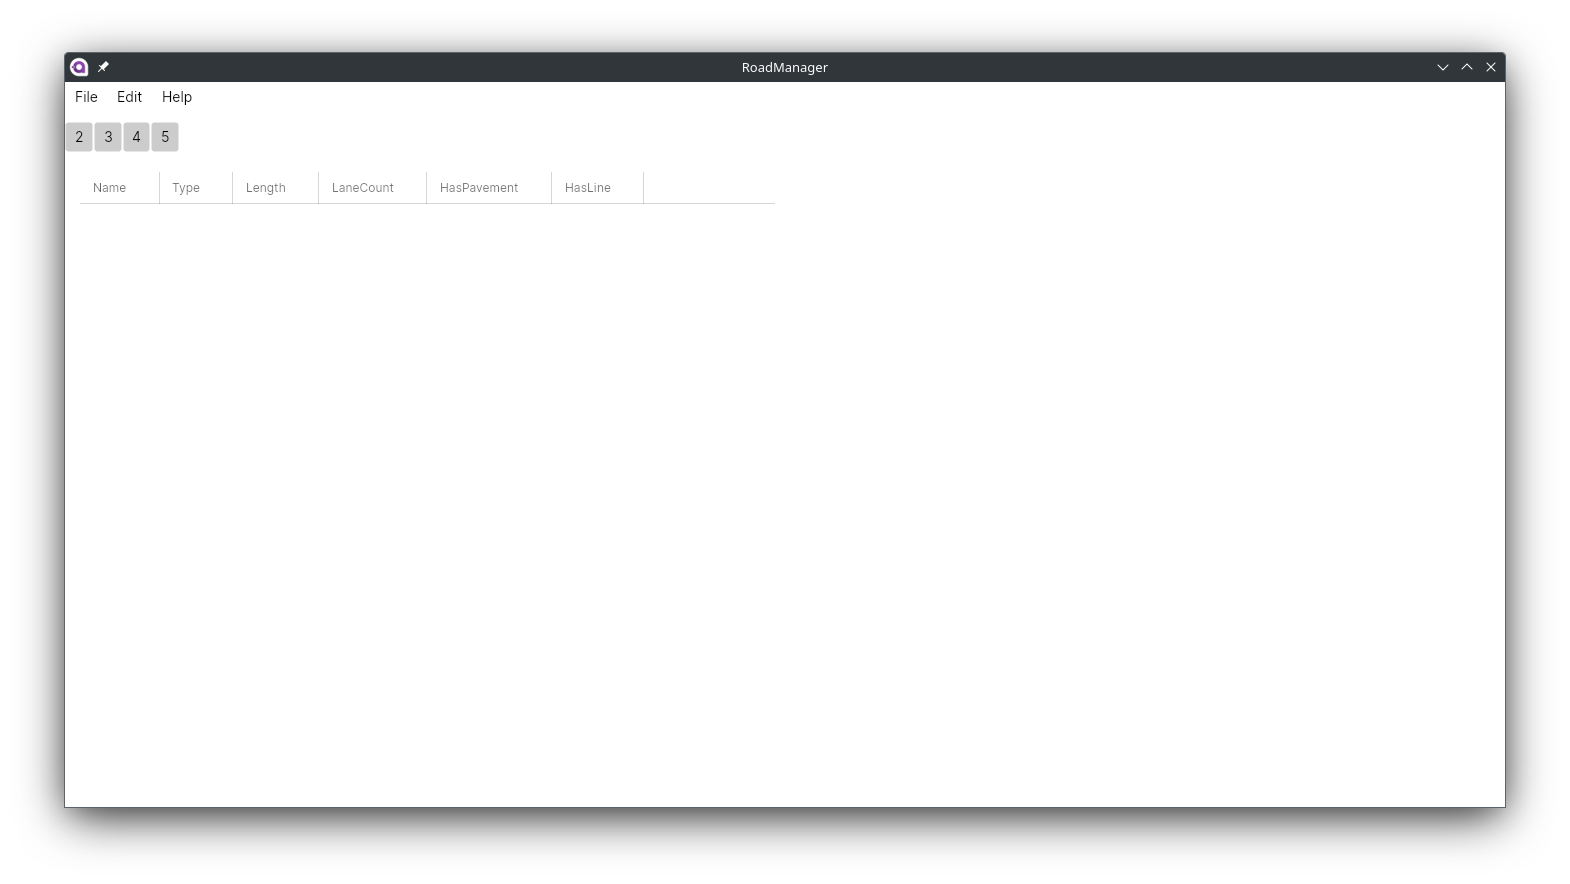
\includegraphics[width=0.90\textwidth]{startup.png}
    \caption{Cтартовий екран / Головне вікно}
\end{figure}
\begin{figure}[H]
    \centering
    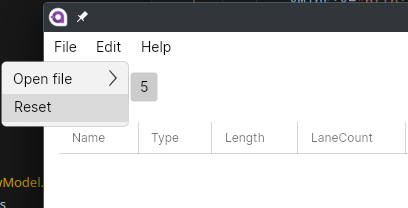
\includegraphics[width=0.90\textwidth]{on_file_click.png}
    \caption{Натискання на кнопку File}
\end{figure}
\begin{figure}[H]
    \centering
    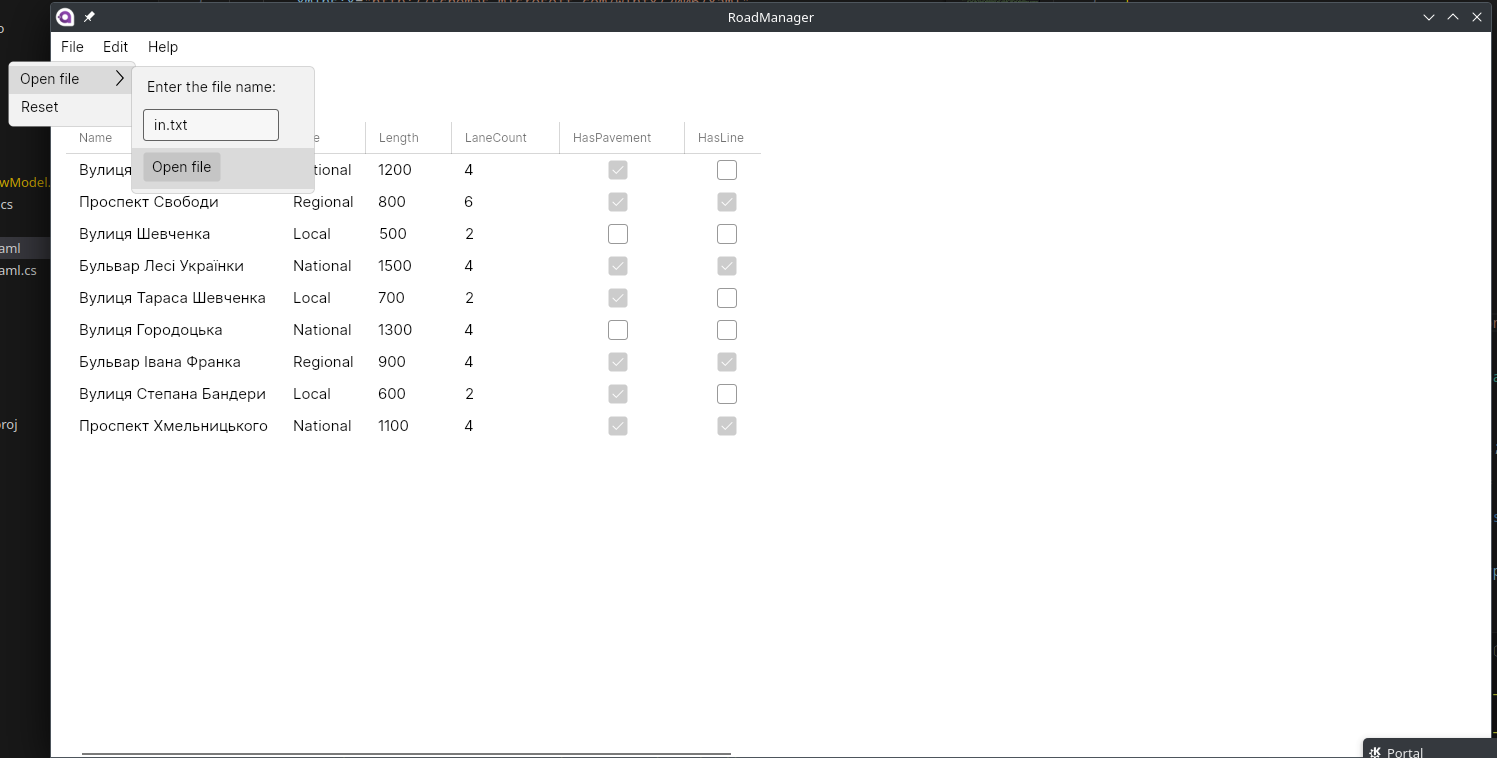
\includegraphics[width=0.90\textwidth]{on_file_open_click_good.png}
    \caption{Натискання на Open file}
\end{figure}
\begin{figure}[H]
    \centering
    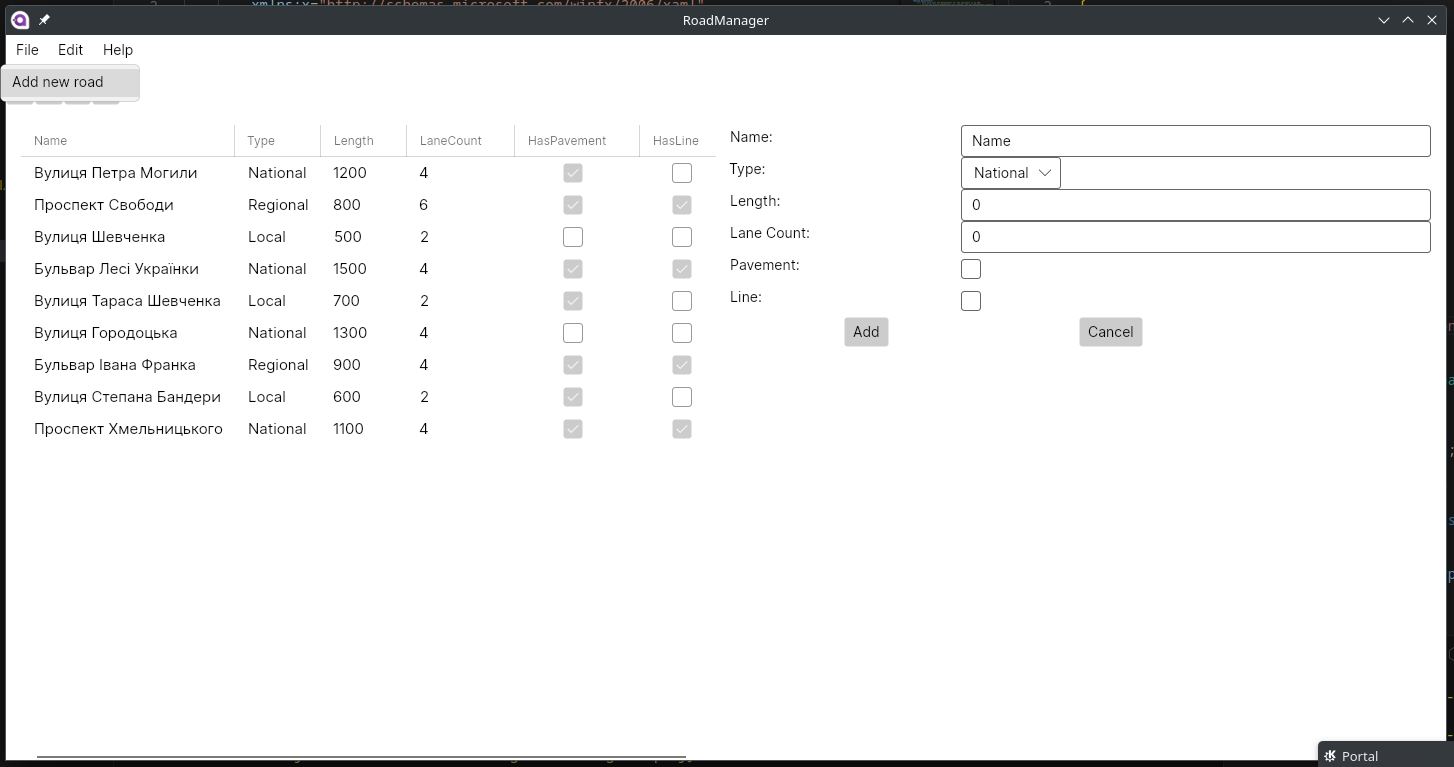
\includegraphics[width=0.90\textwidth]{add_road_click.png}
    \caption{Натискання на меню Edit і кнопку Add new road}
\end{figure}
\begin{figure}[H]
    \centering
    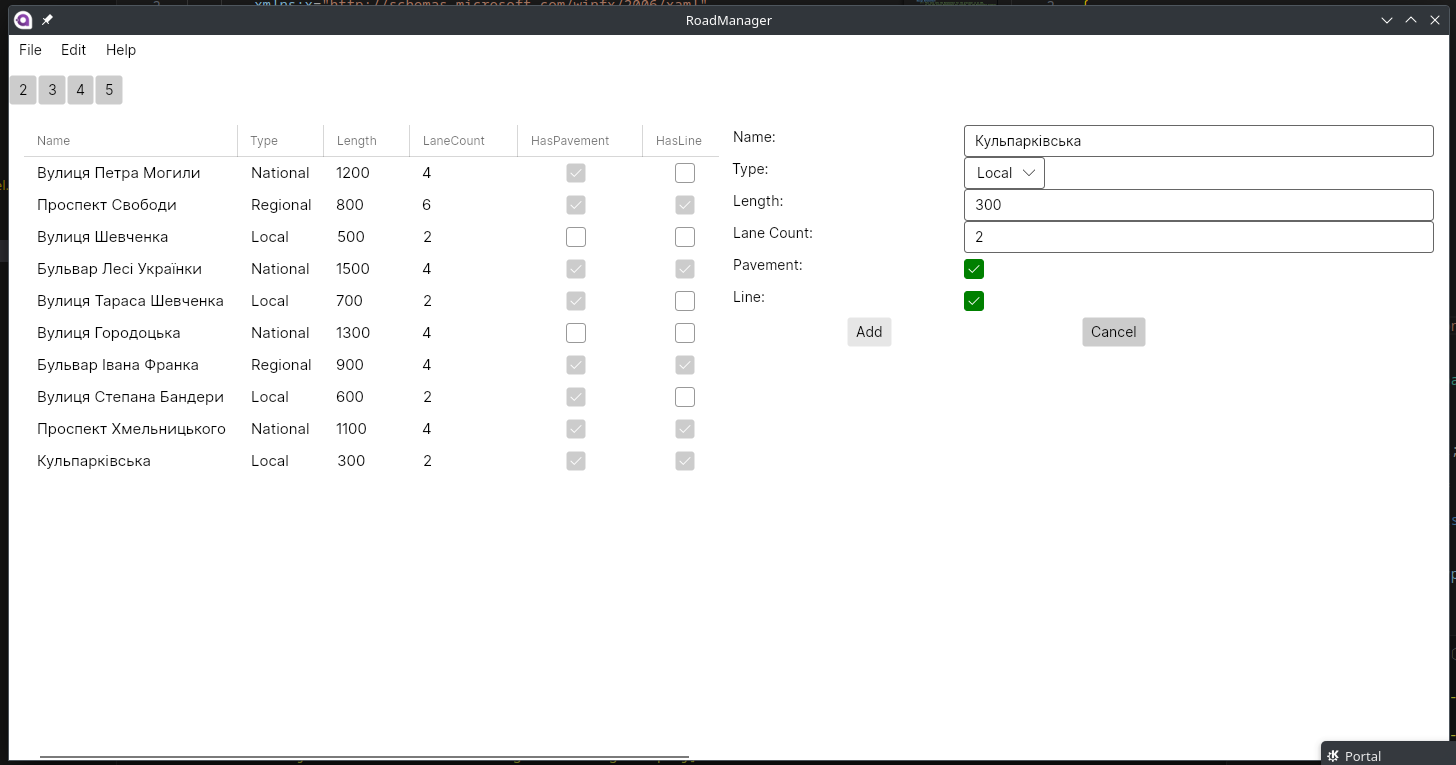
\includegraphics[width=0.90\textwidth]{add_road_result.png}
    \caption{Введення даних в поля зправа}
\end{figure}
\begin{figure}[H]
    \centering
    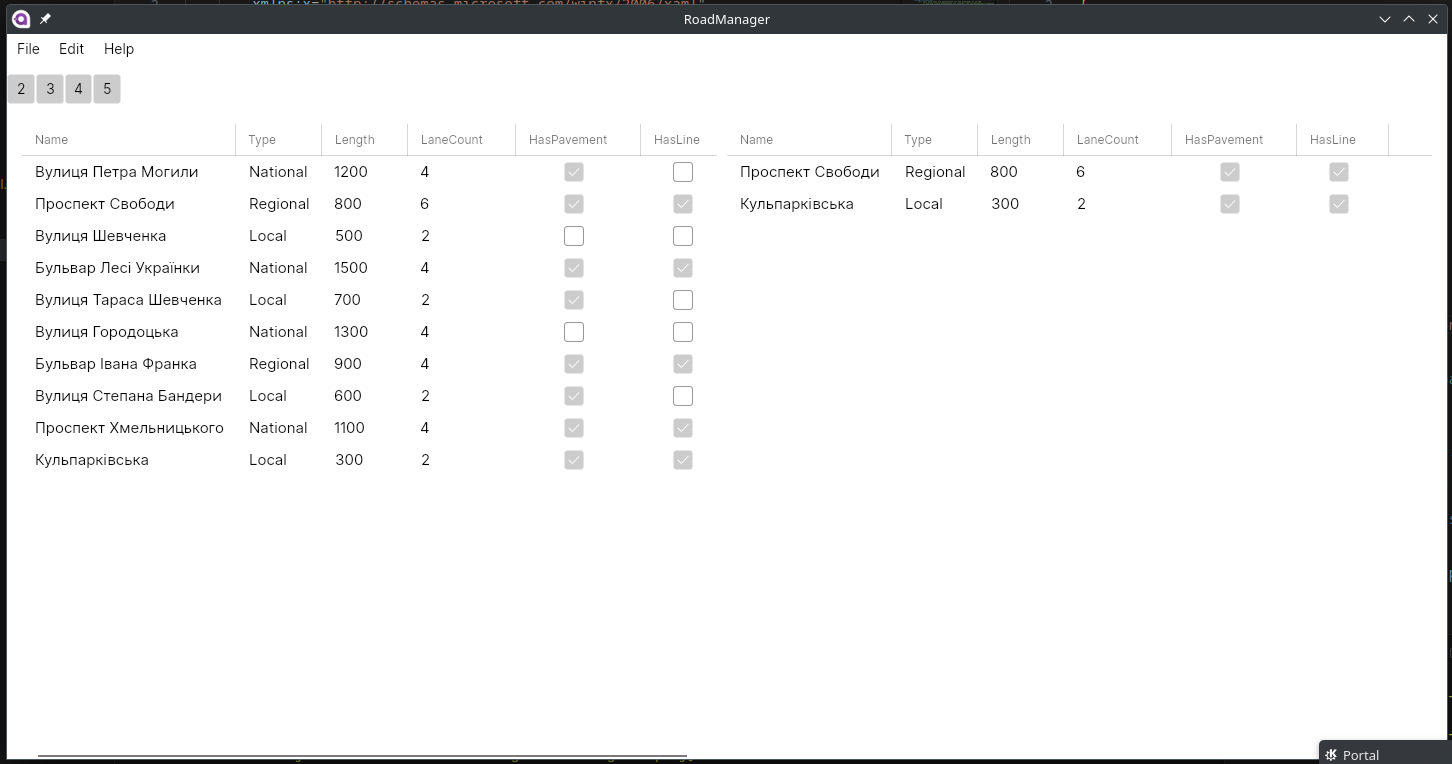
\includegraphics[width=0.90\textwidth]{second_task.png}
    \caption{Натискання на кнопку 2}
\end{figure}
\begin{figure}[H]
    \centering
    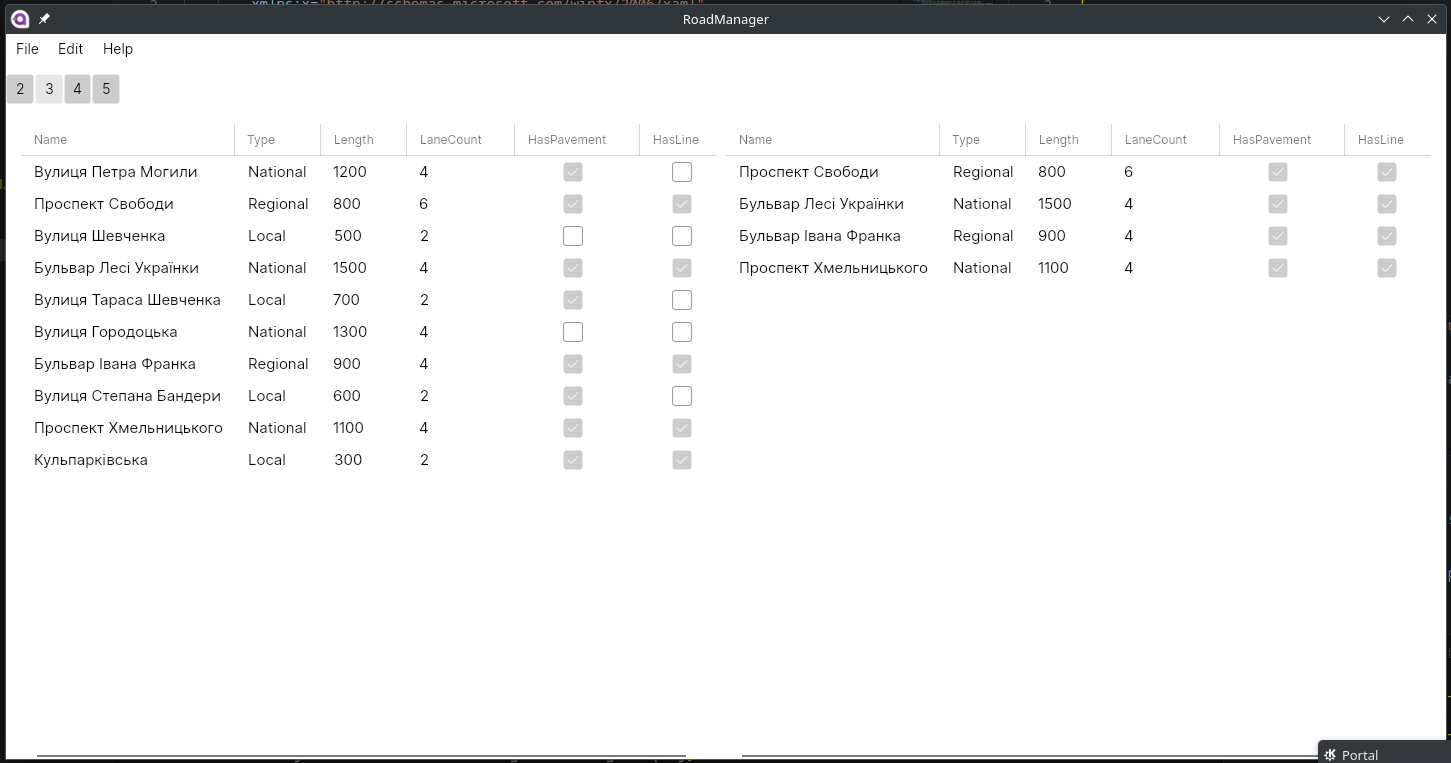
\includegraphics[width=0.90\textwidth]{task3.png}
    \caption{Натискання на кнопку 3}
\end{figure}
\begin{figure}[H]
    \centering
    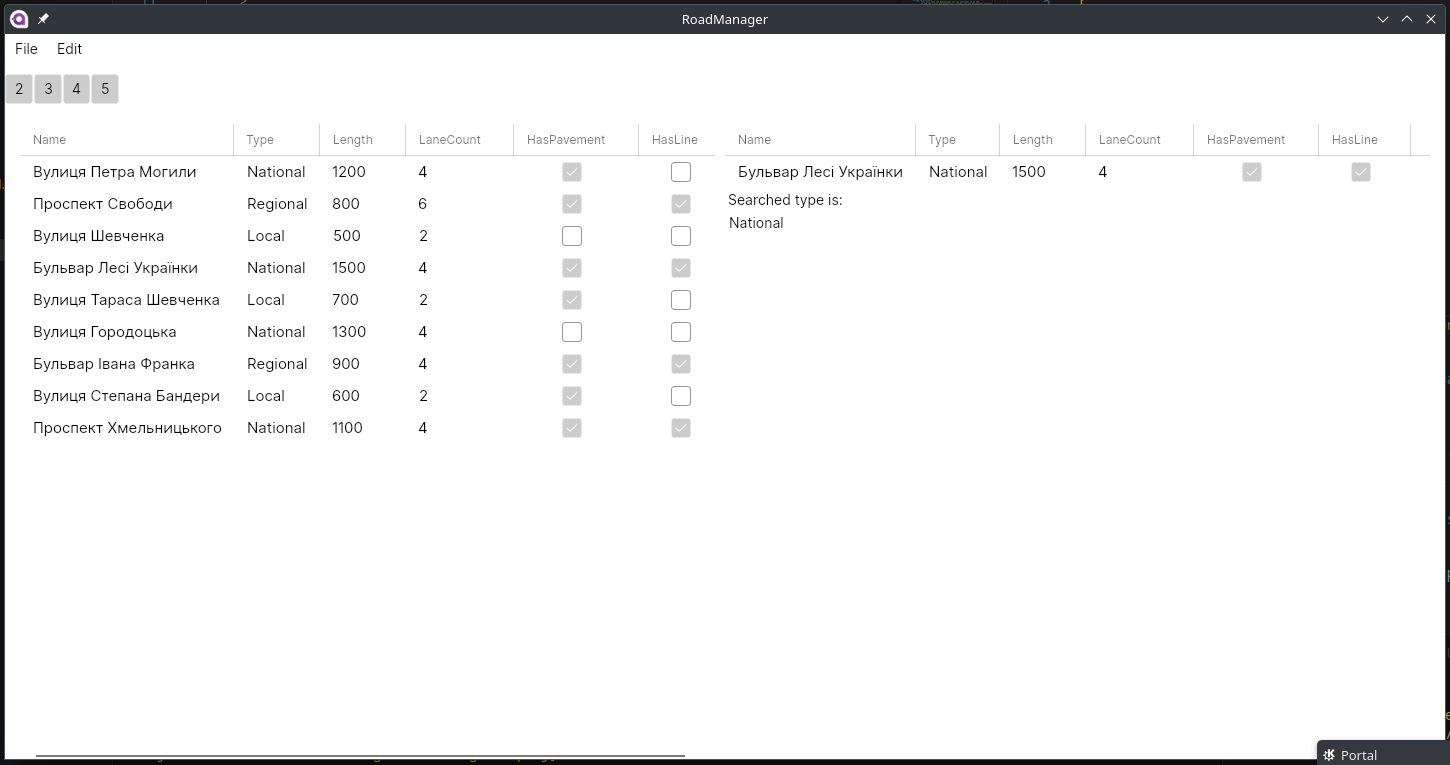
\includegraphics[width=0.90\textwidth]{task4.png}
    \caption{Натискання на кнопку 4}
\end{figure}
\begin{figure}[H]
    \centering
    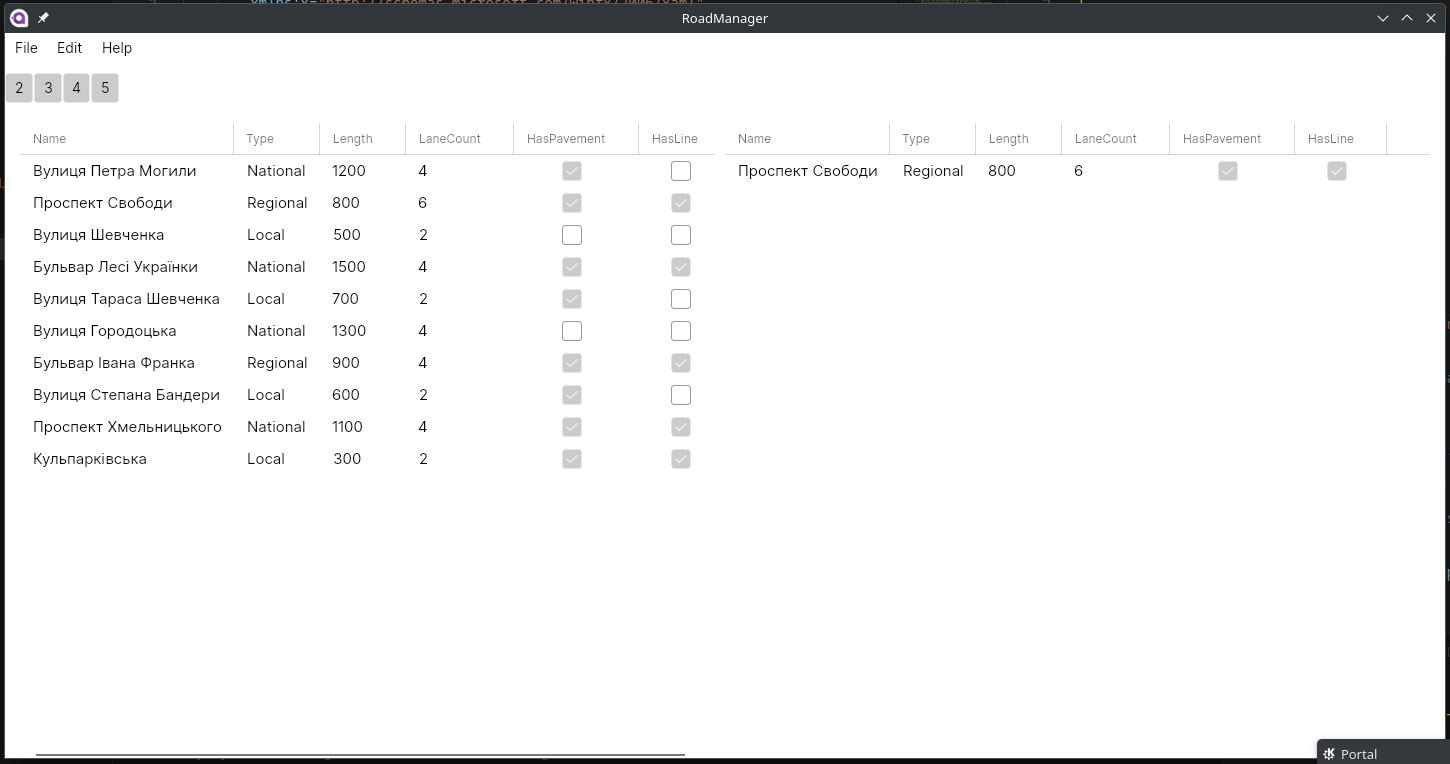
\includegraphics[width=0.90\textwidth]{task5.png}
    \caption{Натискання на кнопку 5}
\end{figure}

\section{Інструкція користувача та системні вимоги}

\subsection{Встановлення ПЗ}

Додаток створений за допомогою .NET тому для його запуску достатньо мати об'єктний файл програми
та встановлений dotnet-runtime або ASPNET.

\subsection{Налаштування ПЗ}

Налаштування додатку користувачем не передбачається.

\subsection{Посібник Користувача Додатку Менеджер Доріг}

\begin{enumerate}
    

\item    Відкриття Додатку:
        \begin{itemize}
            
        \item Запустіть додаток "Менеджер Доріг".
        \end{itemize}

\item    Інтерфейс Головного Вікна:
        \begin{itemize}
        \item При відкритті ви побачите головне вікно програми.
        \item Воно відображає різні елементи, такі як кнопки, сітки і, можливо, таблицю з інформацією про дороги.
        \end{itemize}

\item    Додавання Дороги:
        \begin{itemize}
        \item Для додавання дороги натисніть на меню "Edit".
        \item З випадаючого меню оберіть "Add Road".
        Ця дія може викликати вспливаюче вікно або область введення, де ви можете ввести деталі про дорогу, такі як її назва, тип, довжина, кількість смуг, наявність покриття і лінії. Введіть необхідну інформацію і натисніть "Save" або еквівалент для додавання дороги.
        \end{itemize}

\item    Перегляд Доріг:
        \begin{itemize}
        \item Основний інтерфейс може відображати список або таблицю, де показана інформація про дороги.
        \item Кожен запис про дорогу може відображати її назву, тип, довжину, кількість смуг, наявність покриття і лінії у окремих колонках.
        \end{itemize}

\item    Пошук Конкретних Доріг:
        \begin{itemize}
        \item Можуть бути кнопки або опції для знаходження доріг за конкретними умовами, наприклад, найдовша дорога із найбільшою кількістю смуг, дороги, що відповідають певним критеріям або найдовша дорога з покриттям.
        \item Клацніть на ці опції, щоб виконати відповідний пошук.
        \end{itemize}

\item    Завантаження Доріг з Файлу:
        \begin{itemize}
        \item Може бути опція для завантаження доріг із файлу.
        \item Клацніть на "Load from File" або схожу кнопку, щоб відкрити діалогове вікно вибору файлу.
        \item Виберіть відповідно структурований файл із інформацією про дороги. Це може бути файл у форматі CSV.
        \end{itemize}

\item    Вихід з Додатку:
        \begin{itemize}
        \item Для виходу з програми просто закрийте головне вікно або використайте будь-яку доступну кнопку "Exit" або "Close".
        \end{itemize}

\item    Додаткові Функції:
        \begin{itemize}
        \item Додаток може мати додаткові функції, такі як сортування доріг, фільтрація або відображення конкретних деталей доріги при кліці на запис.
        \end{itemize}

\item    Обробка Помилок:
        \begin{itemize}
        \item У випадку помилок або несподіваної поведінки додаток може показувати повідомлення про помилки або попередження, щоб користувач зміг зрозуміти, як вирішити проблему.
        \end{itemize}
\end{enumerate}

Запам'ятайте, кроки можуть трохи відрізнятися в залежності від конкретної реалізації та дизайну інтерфейсу додатку "Менеджер Доріг", який ви використовуєте.

\section{Опис виняткових ситуацій}
\subsection{FileNameException}
\begin{figure}[H]
    \centering
    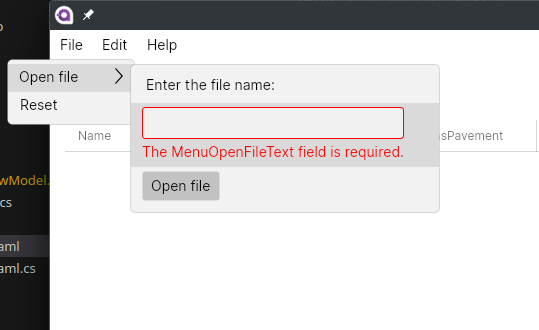
\includegraphics[width=0.90\textwidth]{on_file_open_click_exception.png}
    \caption{Поле імені має бути обов'язково введено}
\end{figure}
\subsection{NameException}
\begin{figure}[H]
    \centering
    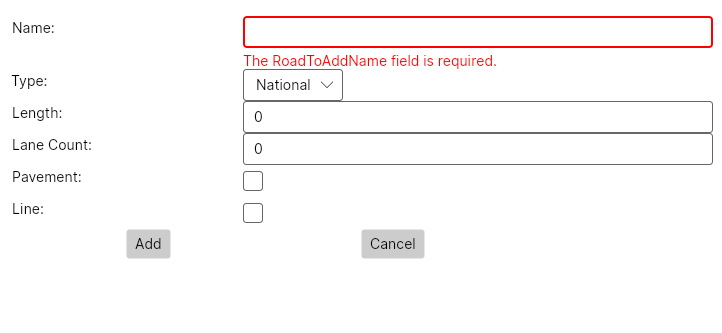
\includegraphics[width=0.90\textwidth]{name_exception.png}
    \caption{Поле імені має бути обов'язково введено}
\end{figure}
\subsection{LengthException}
\begin{figure}[H]
    \centering
    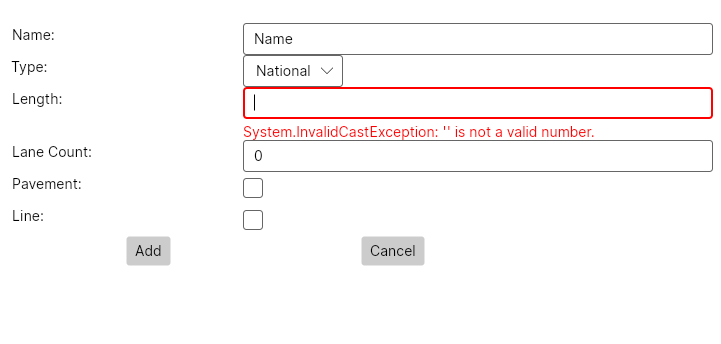
\includegraphics[width=0.90\textwidth]{length_exception.png}
    \caption{Поле протяжності має бути більше нуля}
\end{figure}
\subsection{LaneCountException}
\begin{figure}[H]
    \centering
    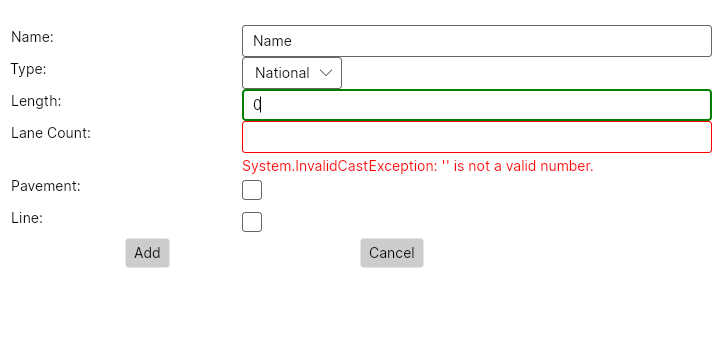
\includegraphics[width=0.90\textwidth]{lane_exception.png}
    \caption{Поле кількості смуг має бути більше нуля}
\end{figure}

\section{Структура файлу вхідних даних}
Програма має змогу зчитувати інформацію з двох типів файлів - .csv (Comma-separated Values) та .txt (Text). Система вибору файлу на ввід дозволяє користувачу вибрати файл через системний інтерфейс. Програма сприймає кожен рядок як дані для окремої машини, при тому, що поля машини розділені наступним чином:

Назва,Тип,Довжина,КількістьСмуг,НаявністьТротуару, НаявністьРозділювальноїСмуги

Зчитування передбачає, що після коми відсутні пробіли, якщо ж присутні – програма автоматично їх вилучає.

Назва і тип це стрічки, довжина і кількість смуг цілі числа, наявність тротуару та розділювальної смуги це булеві значення що задаються ключовими словами false i true

\begin{figure}[H]
    \centering
    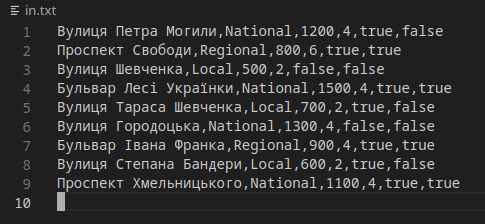
\includegraphics[width=0.90\textwidth]{csv}
    \caption{Поле кількості смуг має бути більше нуля}
\end{figure}
\section{Висновки}
У результаті виконання курсової роботи мною було закріплено основні 
принципи та можливості об'єктно орієнтованого програмування. Для цього 
я спроєктував та розробив програмне забезпечення для класу Машина. 
Для проєктування програми мною було застосовано знання з дисципліни 
«Інженерія програмного забезпечення», а саме: евристики написання 
програмного інтерфейсу, UML-діаграми для зображення архітектури
 програми, стандарти написання коду та тестування програми. 
У реалізації задумки було використано мову програмування C Sharp, 
що ідеально підходить для вивчення та застосування принципів об'єктно 
орієнтованого програмування. Для побудови зовнішьного вигляду програми
 та взаємодії користувача з нею мною було використано Avalonia UI, це 
 кросплатформенний фреймворк для графічних інтерфейсів.
Серед особливостей об’єктно орієнтованого підходу у моєму програмному 
забезпеченні було використано зокрема: створення користувацьких класів,
 полів, методів, конструкторів, статичних варіацій цих частин програми. 
 Також, особливістю C Sharp є те, що всі стандартні та користувацькі змінні 
 повинні бути або структурами, або класами, тобто навіть найменші змінні
  у програмі підтримують об’єктно орієнтований підхід, мають власні 
  методи, тощо. Я ознайомився з такою особливістю і повністю застосував
   її у програмі.
У підсумку поступового проєктування та реалізації програмного 
забезпечення було створено фінальну програму з повноцінною взаємодією к
ористувача; передбаченими за допомогою механізму обробки об’єктів
 «Винятків» обробкою критичних ситуацій; можливістю отримати 
 інструкцію користувача через інтерфейс програми; реалізованими всіма 
 передбаченими варіантом функціями взаємодії з Машиною.
Також, для зручності вводу було створено два способи зчитування даних: 
через відповідні поля інтерфейсу у програмі через клавіатуру та за
 допомогою файлового зчитування.

\section{Списки використаних джерел}
\begin{enumerate}
    \item Методичні вказіви до виконання курсової роботи з дисципліни «Об'єктно-орієнтоване програмування» для студентів першого (бакалаврського) рівня вищої освіти, напряму 121 «Інженерія програмного забезпечення» / Укл.: Коротєєва Т.О., Дяконюк Л.М., 27 стор., Сам.видав № 9347, 2020.
    
    \item Є. В. Левус, Т. А. Марусенкова, О. О. Нитребич. Життєвий цикл   
програмного забезпечення / Є. В. Левус, Т. А. Марусенкова, О. О. 
Нитребич. - Львів : Видавництво Львівської політехніки, 2017.-  208 с.
    \item \verb*|C#| 8.0 and .NET Core 3.0 – Modern Cross-Platform Development: Build applications with \verb|C#|, .NET Core, Entity Framework Core, ASP.NET Core, and ML.NET using Visual Studio Code, 4th Edition/Mark J. Price.- Packt Publishing,2019.-818с.
    \item \verb|С#| For Beginners: An Introduction to \verb|C#| Programming with Tutorials and Hands-On Examples/Nathan Metzler.,2018.-73p.
    \item \verb|C#| in Depth: Fourth Edition 4th Edition/Jon Skeet-Manning Publications.,2019.- 528 с
    \item Scott Meyers. Effective STL / AddisonWesley, an imprint of Pearson Education, Inc. – 60p. 
\end{enumerate}


\end{document}